\documentclass[compact]{beamer}%handout
\usepackage[utf8]{inputenc}
\usetheme{Warsaw}


\mode<handout> {
	\usepackage{handoutWithNotes}
	\pgfpagesuselayout{2 on 1 with notes landscape}[a4paper,border shrink=5mm]
}
	
\setbeamertemplate{navigation symbols}{} 
\useoutertheme{infolines}
\setbeamertemplate{footline}
{%
  \leavevmode%
  \hbox{\begin{beamercolorbox}[wd=.5\paperwidth,ht=2.5ex,dp=1.125ex,leftskip=.3cm plus1fill,rightskip=.3cm]{author in head/foot}%
    \usebeamerfont{author in head/foot}\insertshortauthor
  \end{beamercolorbox}%
  \begin{beamercolorbox}[wd=.41\paperwidth,ht=2.5ex,dp=1.125ex,leftskip=.3cm,rightskip=.3cm plus1fil]{title in head/foot}%
    \usebeamerfont{title in head/foot}\insertshorttitle 
  \end{beamercolorbox}%
  \begin{beamercolorbox}[wd=.09\paperwidth,ht=2.5ex,dp=1.125ex,leftskip=.3cm plus1fill,rightskip=.3cm]{author in head/foot}%
    \usebeamerfont{author in head/foot}\insertframenumber/\inserttotalframenumber
  \end{beamercolorbox}}%
  \vskip0pt%
}

\AtBeginSection[]{
  \begin{frame}{Sommaire}
  \small \tableofcontents[currentsection, hideothersubsections]
  \end{frame} 
}


\definecolor{fontcolor}{rgb}{0.92,0.92,0.99}
\usepackage{listings}
\lstset{language=Java, numbers=left, tabsize=2, frame=single, breaklines=true,  numberstyle=\tiny\ttfamily,basicstyle=\small, framexleftmargin=5mm, backgroundcolor=\color{fontcolor}, xleftmargin=5mm, basicstyle=\tiny }

\graphicspath{images}

\title{Référentiel Coordonnées JAVA}
\subtitle{Architecture et solutions techniques}
\author{Thomas Duchatelle (thomas.duchatelle-ext@yrnet.com)}
\institute{Yves Rocher}


%%%%%%%%%%%%%%%%%%%%%%%%%%%%%%%%%%%%%%%%%%%%
%% DOCUMENT
%%%%%%%%%%%%%%%%%%%%%%%%%%%%%%%%%%%%%%%%%%%%
\begin{document}


% Pages de présentations...
\frame{\titlepage}
  
\section*{Plan}
\frame{\tableofcontents[hideallsubsections]}
	
%%%%%%%%%%%%%%%%%%%%%%%%%%%%%%%%%%%%%%%%%
%% ARCHITECTURE
\section{Architecture générale}

\subsection{Couches applicatives et modules}

\begin{frame}{Référentiel Coordonnées}
	\framesubtitle{1 application, 4 modules}

	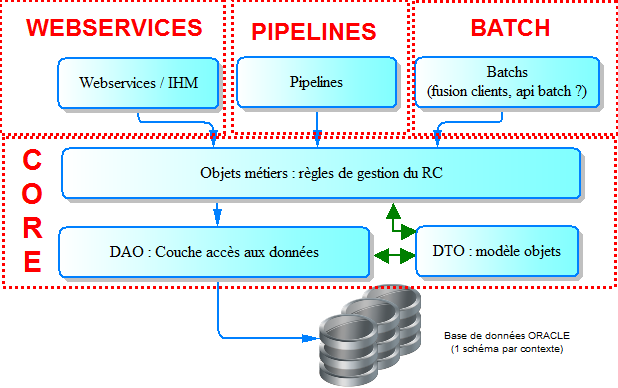
\includegraphics[width=\textwidth]{images/rc_arch_general.png}
\end{frame}

\begin{frame}{Modules du référentiel coordonnées}
	\begin{description}[<+->]
	\item[Core] Coeur de l'application (jar) :
		\begin{itemize}
		\item Modèle objets : représentation \emph{client} / \emph{coordonnées}
		\item couche d'accès au données : structure de la base, gestion des schémas
		\item règles de gestion : calcul des consentements, règles de mises à jour, dé-duplication
		\end{itemize}
	\item[Webservices] Application Java EE (war) exposant des webservices
		\begin{itemize}
		\item correspondance \emph{modèle objet interne} $\leftrightarrow$ \emph{contrat WSDL}
		\item Interface WEB : suivi des pipelines
		\end{itemize}
	\item[Pipelines] Intégration de données par fichiers CSV
		\begin{itemize}
		\item Démarrage/Arrêt d'un \emph{démon}
		\item Détection de l'arrivée de fichiers
		\item EAI et lecture de fichier
		\item Parallélisation des traitements
		\end{itemize}
	\item[Batch] Exports, traitements types fusion, statistiques
	\end{description}
\end{frame}


\begin{frame}{Organisation du code}
	
	\begin{block}{Maven}
	Le référentiel coordonnées utilise \emph{Maven} pour : 
	\begin{itemize}
	\item la gestion des dépendances
	\item la compilation 
	\item le déploiement des pipelines et batch
	\item configuration du poste de travail : \emph{Eclipse}\par
	(1 projet maven = 1 projet Eclipse)
	\item tests en local des webservices et IHM
	\end{itemize}
	\end{block}
	
	\pause
	\begin{block}{Projets Maven}
	Chaque modules du RC est représenté par un sous-projet Maven.
	\end{block}

\end{frame}

\begin{frame}{Projets et sous-projets \emph{Maven}}
	
	Le référentiel coordonnées est répartie sur 6 projets \emph{Maven} :
	\begin{itemize}[<+->]
	\item \textbf{addressrepository} : \emph{version, déclarations des dépendances}
		\begin{itemize}
		\item \textbf{address-core} : \emph{coeur de l'application}\par
		package : \texttt{net.yvesrocher.services.address.core}
		\item \textbf{address-pipelines} : \emph{Jar exécutable (démon)}\par
		package : \texttt{net.yvesrocher.services.address.pipelines}
		\item \textbf{address-webservices} : \emph{War du webservices}\par
		package : \texttt{net.yvesrocher.services.address.webservices}
		\item \textbf{address-ear} : \emph{Package le war en un EAR}
		\item \textbf{address-batch} : \emph{Batchs utilisant le coeur V3, jar exécutable}\par
		package : \texttt{net.yvesrocher.services.address.batch}
		\end{itemize}
	\end{itemize}

\end{frame}

\subsection{Outils utilisés}

\begin{frame}{Outils et frameworks utilisés}

	\begin{description}
	\item[Spring] Inversion de contrôle, gestion des contextes, transactions BDD
	\item[Hibernate] \emph{Mapping Relationnel Objet}
	\item[Hibernate Validator] Validation des données
	\item[SLF4J] API de log, utilise \emph{LOG4J} en backend
	\item[Commons Apache] Utilitaires sur les chaines de caractères, la détection des fichiers, ...
	\item[JUNIT] Tests unitaires (utilisé avec \emph{Mockito} et \emph{FestAssert})
	\end{description}
	
\end{frame}

\subsection{Compilation et déploiement}

\begin{frame}{Compilation et déploiement}

	\begin{block}{Compilation}
	Maven exécute les tests unitaires et crée les binaires s'il n'y a pas d'erreur. Les binaires sont présents dans le répertoire \texttt{target} de chaque module.
	\end{block}
	
	\pause
	Commande Maven de compilation et déploiement sur FTP :
	\begin{lstlisting}
mvn clean install -DdeployPipelines
	\end{lstlisting}

\end{frame}


\section{Coeur applicatif}

\subsection{Couche d'accès au données}

\begin{frame}{Cartographie du coeur}

\end{frame}
% Pattern "open session in view"
% Scope "context"

\subsection{Plan et principales briques logicielles}

\subsection{API de tests unitaires}
% @DatabaseScripts

\section{Webservices et IHM}

% parler des bean de mappers
% CXF
% Spring MVC

\section{Pipelines}

% configuration
% timers
% plan des beans
% Exemple concret (diagrammes séquence)




\end{document}